%%%%%%%%%%%%%%%%%%%%%%%%%%%%%%%%%%%%%%%%%
% Wenneker Article
% LaTeX Template
% Version 2.0 (28/2/17)
%
% This template was downloaded from:
% http://www.LaTeXTemplates.com
%
% Authors:
% Vel (vel@LaTeXTemplates.com)
% Frits Wenneker
%
% License:
% CC BY-NC-SA 3.0 (http://creativecommons.org/licenses/by-nc-sa/3.0/)
%
%%%%%%%%%%%%%%%%%%%%%%%%%%%%%%%%%%%%%%%%%

%----------------------------------------------------------------------------------------
%	PACKAGES AND OTHER DOCUMENT CONFIGURATIONS
%----------------------------------------------------------------------------------------

\documentclass[10pt, a4paper, twocolumn]{article} % 10pt font size (11 and 12 also possible), A4 paper (letterpaper for US letter) and two column layout (remove for one column)

%%%%%%%%%%%%%%%%%%%%%%%%%%%%%%%%%%%%%%%%%
% Wenneker Article
% Structure Specification File
% Version 1.0 (28/2/17)
%
% This file originates from:
% http://www.LaTeXTemplates.com
%
% Authors:
% Frits Wenneker
% Vel (vel@LaTeXTemplates.com)
%
% License:
% CC BY-NC-SA 3.0 (http://creativecommons.org/licenses/by-nc-sa/3.0/)
%
%%%%%%%%%%%%%%%%%%%%%%%%%%%%%%%%%%%%%%%%%

%----------------------------------------------------------------------------------------
%	PACKAGES AND OTHER DOCUMENT CONFIGURATIONS
%----------------------------------------------------------------------------------------

\usepackage[english]{babel} % English language hyphenation

\usepackage{microtype} % Better typography

\usepackage{amsmath,amsfonts,amsthm} % Math packages for equations

\usepackage[svgnames]{xcolor} % Enabling colors by their 'svgnames'

\usepackage[hang, small, labelfont=bf, up, textfont=it]{caption} % Custom captions under/above tables and figures

\usepackage{booktabs} % Horizontal rules in tables

\usepackage{lastpage} % Used to determine the number of pages in the document (for "Page X of Total")

\usepackage{graphicx} % Required for adding images

\usepackage{enumitem} % Required for customising lists
\setlist{noitemsep} % Remove spacing between bullet/numbered list elements

\usepackage{sectsty} % Enables custom section titles
\allsectionsfont{\usefont{OT1}{phv}{b}{n}} % Change the font of all section commands (Helvetica)

%----------------------------------------------------------------------------------------
%	MARGINS AND SPACING
%----------------------------------------------------------------------------------------

\usepackage{geometry} % Required for adjusting page dimensions

\geometry{
	top=1cm, % Top margin
	bottom=1.5cm, % Bottom margin
	left=2cm, % Left margin
	right=2cm, % Right margin
	includehead, % Include space for a header
	includefoot, % Include space for a footer
	%showframe, % Uncomment to show how the type block is set on the page
}

\setlength{\columnsep}{7mm} % Column separation width

%----------------------------------------------------------------------------------------
%	FONTS
%----------------------------------------------------------------------------------------

\usepackage[T1]{fontenc} % Output font encoding for international characters
\usepackage[utf8]{inputenc} % Required for inputting international characters

\usepackage{XCharter} % Use the XCharter font

%----------------------------------------------------------------------------------------
%	HEADERS AND FOOTERS
%----------------------------------------------------------------------------------------

\usepackage{fancyhdr} % Needed to define custom headers/footers
\pagestyle{fancy} % Enables the custom headers/footers

\renewcommand{\headrulewidth}{0.0pt} % No header rule
\renewcommand{\footrulewidth}{0.4pt} % Thin footer rule

\renewcommand{\sectionmark}[1]{\markboth{#1}{}} % Removes the section number from the header when \leftmark is used

%\nouppercase\leftmark % Add this to one of the lines below if you want a section title in the header/footer

% Headers
\lhead{} % Left header
\chead{\textit{\thetitle}} % Center header - currently printing the article title
\rhead{} % Right header

% Footers
\lfoot{} % Left footer
\cfoot{} % Center footer
\rfoot{\footnotesize Page \thepage\ of \pageref{LastPage}} % Right footer, "Page 1 of 2"

\fancypagestyle{firstpage}{ % Page style for the first page with the title
	\fancyhf{}
	\renewcommand{\footrulewidth}{0pt} % Suppress footer rule
}

%----------------------------------------------------------------------------------------
%	TITLE SECTION
%----------------------------------------------------------------------------------------

\newcommand{\authorstyle}[1]{{\large\usefont{OT1}{phv}{b}{n}\color{DarkRed}#1}} % Authors style (Helvetica)

\newcommand{\institution}[1]{{\footnotesize\usefont{OT1}{phv}{m}{sl}\color{Black}#1}} % Institutions style (Helvetica)

\usepackage{titling} % Allows custom title configuration

\newcommand{\HorRule}{\color{DarkGoldenrod}\rule{\linewidth}{1pt}} % Defines the gold horizontal rule around the title

\pretitle{
	\vspace{-30pt} % Move the entire title section up
	\HorRule\vspace{10pt} % Horizontal rule before the title
	\fontsize{32}{36}\usefont{OT1}{phv}{b}{n}\selectfont % Helvetica
	\color{DarkRed} % Text colour for the title and author(s)
}

\posttitle{\par\vskip 15pt} % Whitespace under the title

\preauthor{} % Anything that will appear before \author is printed

\postauthor{ % Anything that will appear after \author is printed
	\vspace{10pt} % Space before the rule
	\par\HorRule % Horizontal rule after the title
	\vspace{20pt} % Space after the title section
}

%----------------------------------------------------------------------------------------
%	ABSTRACT
%----------------------------------------------------------------------------------------

\usepackage{lettrine} % Package to accentuate the first letter of the text (lettrine)
\usepackage{fix-cm}	% Fixes the height of the lettrine

\newcommand{\initial}[1]{ % Defines the command and style for the lettrine
	\lettrine[lines=3,findent=4pt,nindent=0pt]{% Lettrine takes up 3 lines, the text to the right of it is indented 4pt and further indenting of lines 2+ is stopped
		\color{DarkGoldenrod}% Lettrine colour
		{#1}% The letter
	}{}%
}

\usepackage{xstring} % Required for string manipulation

\newcommand{\lettrineabstract}[1]{
	\StrLeft{#1}{1}[\firstletter] % Capture the first letter of the abstract for the lettrine
	\initial{\firstletter}\textbf{\StrGobbleLeft{#1}{1}} % Print the abstract with the first letter as a lettrine and the rest in bold
}

%----------------------------------------------------------------------------------------
%	BIBLIOGRAPHY
%----------------------------------------------------------------------------------------

\usepackage[backend=bibtex,style=authoryear,natbib=true]{biblatex} % Use the bibtex backend with the authoryear citation style (which resembles APA)

\addbibresource{example.bib} % The filename of the bibliography

\usepackage[autostyle=true]{csquotes} % Required to generate language-dependent quotes in the bibliography

%%%%%%%%%%%%%%% CODE SNIPPET
\usepackage{listings}
\usepackage{color}

\usepackage{graphicx}
\usepackage{subcaption}

\definecolor{dkgreen}{rgb}{0,0.6,0}
\definecolor{gray}{rgb}{0.5,0.5,0.5}
\definecolor{mauve}{rgb}{0.58,0,0.82}

\lstset{frame=tb,
  language=Java,
  aboveskip=3mm,
  belowskip=3mm,
  showstringspaces=false,
  columns=flexible,
  basicstyle={\small\ttfamily},
  numbers=none,
  numberstyle=\tiny\color{gray},
  keywordstyle=\color{blue},
  commentstyle=\color{dkgreen},
  stringstyle=\color{mauve},
  breaklines=true,
  breakatwhitespace=true,
  tabsize=3
}
%%%%%%%%%%%%%%% END CODE SNIPPET
\usepackage{hyperref}
\hypersetup{
    colorlinks=true,
    linkcolor=blue,
    filecolor=magenta,
    urlcolor=cyan,
}
 % Specifies the document structure and loads requires packages

%----------------------------------------------------------------------------------------
%	ARTICLE INFORMATION
%----------------------------------------------------------------------------------------

\title{Introduction to Nim} % The article title

\author{
	\authorstyle{Boitumelo Phetla} % Authors
	\newline\newline % Space before institutions
	\textsuperscript{1}\institution{General-purpose Programming Language}\\ % Institution 1
}

% Example of a one line author/institution relationship
%\author{\newauthor{John Marston} \newinstitution{Universidad Nacional Autónoma de México, Mexico City, Mexico}}

\date{\today} % Add a date here if you would like one to appear underneath the title block, use \today for the current date, leave empty for no date

%----------------------------------------------------------------------------------------

\begin{document}

\maketitle % Print the title

\thispagestyle{firstpage} % Apply the page style for the first page (no headers and footers)

%----------------------------------------------------------------------------------------
%	ABSTRACT
%----------------------------------------------------------------------------------------

\lettrineabstract{Nim is unique. It is multi-paradigm, general purpose programming language with syntax like Python. However, the language or the design of this programming language does not emphasize on Object Oriented Programming style/concept. The language follows its own programming styling, it is imperative that its syntax styling is kept as guided by Nim's reference manual. Nim focuses mainly on effiency, expressiveness, and elegance. Nim is much like any other programming language with features such as concurrency, parallelism, user-defined types, the standard library, and more. Nim also has Nim's specific features such as asynchronous input/output, metaprogramming, and the foreign function interface.}

%----------------------------------------------------------------------------------------
%	ARTICLE CONTENTS
%----------------------------------------------------------------------------------------

\section{What is Nim?}

\begin{figure}[hbt!]
	
\includegraphics[width=0.25\linewidth]{Nim.png} % Figure image
	%\caption{Nim} % Figure caption
	\label{nim} % Label for referencing with \ref{bear}
\end{figure}

Impatience is my vice, I want to know I have the right tools for the job before I commit. So what does this mean?
\\
\\
\textbf{\href{https://exercism.io/tracks/nim/installation}{How to install Nim}}
\\
\begin{lstlisting}
$bash: brew install nim

==> Pouring nim-0.19.4.mojave.bottle.tar.gz
/usr/local/Cellar/nim/0.19.4: 411 files, 12.8MB
\end{lstlisting}
\newpage
\textbf{Simple Script}
\\
\\
Create file hello\_world.nim
\begin{lstlisting}
#simple comment line
echo "Hello world!"
\end{lstlisting}
\\
\\
\textbf{Compile Script}
\\
\\
Compile hello\_world.nim
\begin{lstlisting}
$bash: nim compile --run hello_world.nim
Hint: used config file '/usr/local/Cellar/nim/0.19.4/nim/config/nim.cfg' [Conf]
Hint: system [Processing]
Hint: hello_world [Processing]
CC: hello_world
CC: stdlib_system
Hint:  [Link]
Hint: operation successful (12382 lines compiled; 0.660 sec total; 16.383MiB peakmem; Debug Build) [SuccessX]
Hint: /Volumes/pulse/100/Nim/ch01/code/hello_world  [Exec]
Hello world!
\end{lstlisting}
\\
\textbf{Terminal output results}
\\
At this stage I try to understand what the terminal is showing and if I cannot make sense of it, I at least try to find out if my output results is as expected.
\begin{lstlisting}
Hint: used config file '/usr/local/Cellar/nim/0.19.4/nim/config/nim.cfg' [Conf]
		<---- :accessing this directory shows
			  |------ nim.cfg
			  |------ nimdoc.cfg
			  |------ nimdoc.tex.cfg
Hint: system [Processing]
Hint: hello_world [Processing]
CC: hello_world 	<--- looks like Nim is using clang
CC: stdlib_system	<--- looks like Nim is using clang
Hint:  [Link]
Hint: operation successful (12382 lines compiled; 0.660 sec total; 16.383MiB peakmem; Debug Build) [SuccessX] <--- processed Nim packages
Hint: /Volumes/pulse/100/Nim/ch01/code/hello_world  [Exec] <--- script location
Hello world! <--- Expected output
\end{lstlisting}

\textbf{What is in the file/script}

\begin{lstlisting}
In the code repo Nim has created some sort of an object file hello_world (machine code) that Nim (JVM if it is running on it) uses to compile and read the script. Languages such as Java, C, C++ uses such approach (compiled languages). Python does not do such (interpreted language).

$bash: tree -L 1
		hello_world
		hello_world.nim

0 directories, 2 files
\end{lstlisting}

%------------------------------------------------

\subsection{Beginning to learn Nim}

Nim is still a relatively new programming language (first scribbed books ---- Nim in Action, Dominik Picheta).

What should you know going in:
\begin{itemize}
	\item The language is not fully complete
	\item Nim is a general-purpose programming language
	\item effiency, expressiveness and elegance are Nim's standardised priority markers and they rank according to the order mentioned
	\item Nim shares many of Python's characteristics
	\item Nim is a compiled language (translated to C first)
	\item Nim is well suited for systems programming (hardware, OSs, IoT, etc)
	\item Nim is one of the few languages that uses its own language to interpret itself
	\item type system, execution model
	\item Applications that perform I/O operations, such as reading files or sending data over a network, are also well supported by Nim.
	\item Web applications (web frameworks like Jester)
	\item Nim can compile JavaScript
	\item Things that you might be familiar with are covered in Nim (procedures, methods, iterators, generics and templates)
	\item \href{https://github.com/nim-lang/Nim#contributing}{Nim's documentation}
\end{itemize}

\newpage
\subsection{Why should you use Nim}
\begin{description}
	\item[Python, C, C++, ObjC, JavaScript] $\longrightarrow$ Nim's design follows that of Python with the capability to perform foreign interfacing (C, C++, ObjectiveC, JavaScript)
	\item[Nim project started in 2005] $\longrightarrow$  The language is 14 years old, so you will be some sort of an early adopter
	\item[Garbage collector] $\longrightarrow$  Garbage collection + manual memory management
	\item[Game developers] $\longrightarrow$  because of a garbage collector that can be turned on and off this is a useful application for GameDevs
	\item[Scientific computing] $\longrightarrow$  Data Scientists
	\item[Scripting] $\longrightarrow$  Clue codes
	\item[Operating Systems] $\longrightarrow$  Supports Windows, Linux, Unix
	\item[effiency] $\longrightarrow$  Nim focues on compile-time mechanisms (runtime becomes effient)
	\item[Package manager] $\longrightarrow$   Nimble
	\item[Environments to use Nim] $\longrightarrow$  Web applications, Kernel
	\item[Andreas Rumpf] $\longrightarrow$  Andreas Rumpf is the designer of Nimrod programming language, which he develops in his spare time. He is a software engineer working at a top secret company and constantly attempts to create his own start-up which he will allow himself to program in Nimrod full-time. He has programmed in various programming languages over the years (including quite obscure ones) without being satisfied with any of them. Andreas Rumpf holds a degree in Computer Science which he obtained from the University of Kaiserslautern.
\end{description}

\href{https://github.com/nim-lang/Nim#contributing}{The compiler, standard library, and related tools are all open source and written in Nim.}
%------------------------------------------------

\subsection{Core features of Nim}

\begin{enumerate}
	\item Metaprogramming $\longrightarrow$ Read, Generate, Analyze and Transform source code
	\item Style-insensitive $\longrightarrow$ camelCase or snake\_case
	\item Compilation to C $\longrightarrow$ enhances the language's performance
\end{enumerate}

\begin{figure}[h!]
	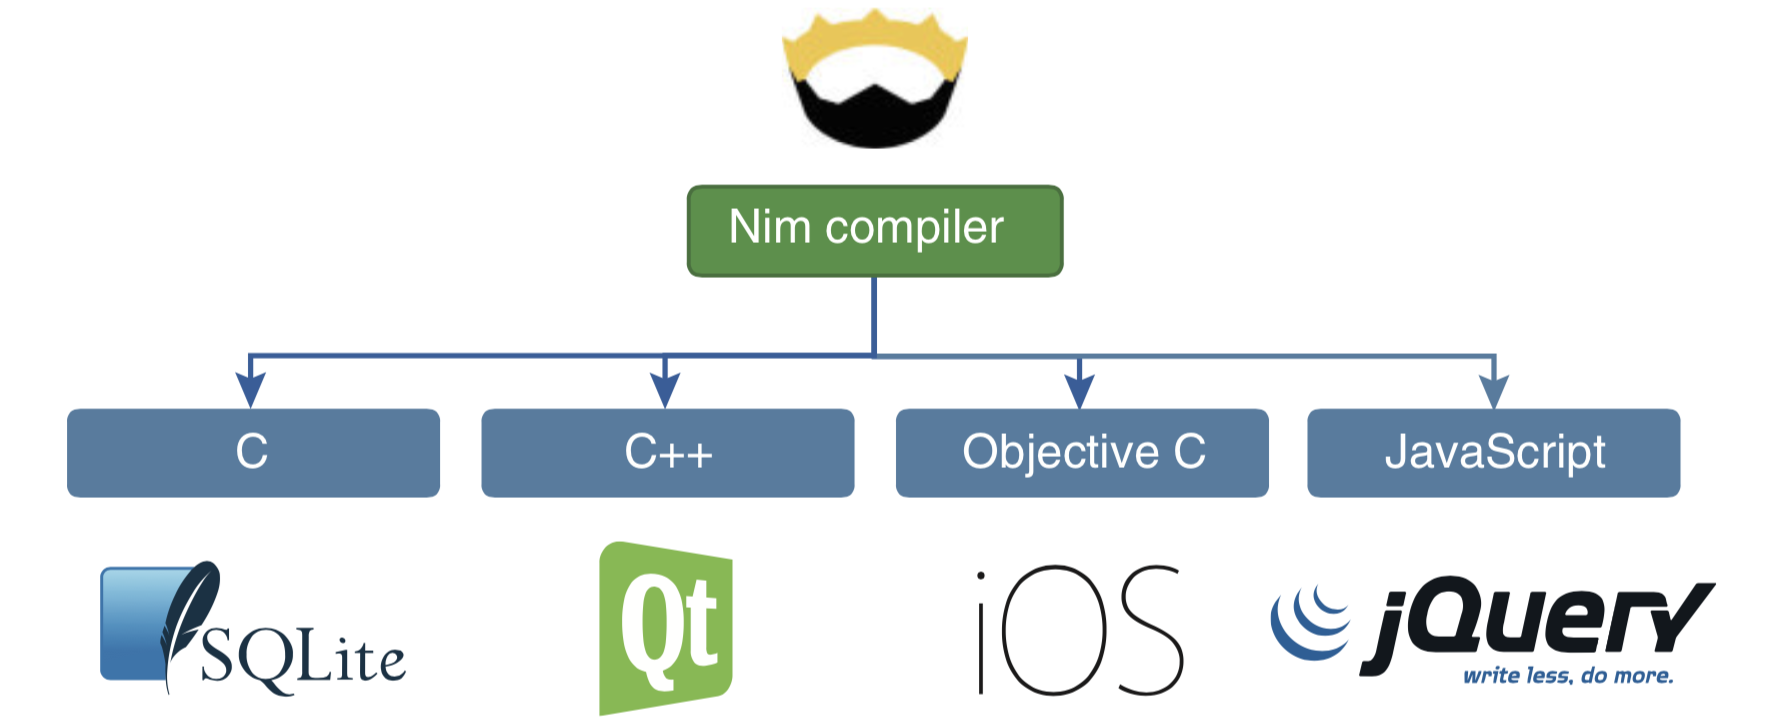
\includegraphics[width=\linewidth]{compiler.png} % Figure image
	\caption{compilers} % Figure caption
	\label{Nim Compilers} % Label for referencing with \ref{bear}
\end{figure}
\newpage

\subsection{Metaprogramming}

Metaprogramming is the writing of computer programs with the ability to treat programs as their data. It means that a program could be designed to read, generate, analyse and/or transform other programs, and even modify itself while running. \textit{Sounds like stuff from the movies}.  \\

\href{https://hookrace.net/blog/introduction-to-metaprogramming-in-nim/}{HookRace blog}


\begin{itemize}
	\item Normal procs and inline iterators
	\item Generic procs  and closure iterators
	\item Templates
	\item Macros
\end{itemize}

With Nim's metaprogramming capabilities you are able to write domain-specific languages (DSL) shown below in simple few lines.

\begin{lstlisting}
echo("<html>")
echo("  <body>")
echo("    <p>Hello World</p>")
echo("  </body>")
echo("</html>")

output:
<html>
  <body>
    <p>Hello World</p>
  </body>
</html>
\end{lstlisting}


\subsubsection{Normal procs (Functions)}

\begin{lstlisting}
#declare function
proc stationName(station: string) =
			echo "Analyzing " , station, " station"

#call function
stationName("Westergloor")      # f(a)
"Azaadville".stationName        # a.f = f(a)
stationName "Mohlakeng"         # f a

output:
Analyzing Westergloor station
Analyzing Azaadville station
Analyzing Mohlakeng station
\end{lstlisting}

\subsubsection{What does style insensitive mean?}

Notice the use of method to\_upper\(\) and toUpper\(\) executes
the same thing, but adopts snake\_case and camelCase.

\begin{lstlisting}
#style insensitive
import strutils

proc nameFormat(fm: string, name: string) =
  if fm == "Y":
    echo "called toUpper() : " , name.toUpper()
  else:
    echo "called to_upper(): " ,name.to_upper()

nameFormat("Y", "john")
nameFormat("N", "john")

output:
called toUpper() : JOHN
called to_upper(): JOHN
\end{lstlisting}

\subsection{Foreign language interface}

\subsubsection{nim compile to JavaScript}
\begin{lstlisting}
nim js -d:nodejs [name of script].nim
\end{lstlisting}

Compiling the code creeates a nimcache directory within the current working directory and generates the JavaScript script in it.

\begin{lstlisting}
tree nimcache
nimcache/
		  |__________  fn1.js
\end{lstlisting}

\subsubsection{nim compile to C}



\begin{lstlisting}
nim -c -d:release c fn1
\end{lstlisting}

The converted C code is stored in the home directory under a hidden file (.cache/nim). It is usually assigned the same name as the nim script name with an suffix underscore some letter.

\begin{lstlisting}
bash$: cd $HOME/.cache/nim
tree 
  |______ fn1_r/
    	     	 |__________ fn1.c
		 		 |__________ fn1.json
		 		 |__________ stdlib_system.c
1 directory, 3 files
\end{lstlisting}

\subsubsection{nim compile to ObjectiveC}

\begin{lstlisting}
nim objc --cpu:amd64 --os:macosx --compile_only --gen_script [script name] 
\end{lstlisting}

The converted objective C code is stored in the home directory under a hidden file (.cache/nim). It is usually assigned the same name as the nim script name with an suffix underscore some letter.

\begin{lstlisting}
fn1_d/
		|__________compile_fn1.sh
		|__________fn1.deps
		|__________fn1.json
		|__________fn1.m
		|__________nimbase.h
		|__________stdlib_system.m
\end{lstlisting}

%-------------------------------------------------------------------------------
%	BIBLIOGRAPHY
%-------------------------------------------------------------------------------

\printbibliography[title={Bibliography}] % Print the bibliography, section title in curly brackets

%------------------------------------------------------------------------------

\end{document}
